\documentclass[a4paper,10pt]{article}

\usepackage[utf8]{inputenc}
\usepackage{graphicx}

\title{Relatorio Trabalho 1}
\author{André Barreto Silveira \\e \\Guilherme Sfalsin Scopel}
\date{03/09/2015}

\pdfinfo{%
  /Title    ()
  /Author   ()
  /Creator  ()
  /Producer ()
  /Subject  ()
  /Keywords ()
}

\begin{document}
\maketitle

 \section{Introdução}
  O trabalho se baseava no problema do "caixero viajante", em que deveriamos encontrar o melhor trajeto possivel (dependendo 
  do algoritimo usado no calculo) entre um conjunto de cidades.
  
  Foram implementados 4 algoritimos para calcular a distancia entre os trajetos, sendo eles o metodo exato(calcula todos os valores 
  de trajetos e compara para descobrir o menor), o vizinho mais proximo(conhecido como NN, verifica o menor valor para a proxima 
  cidade criando o trajeto), opt-2(criado a partir do NN,com melhoramento para indicar um caminho mais perto do melhor caminho possível),
  e o Convex Hull (objetiva gerar o menor polígono que englobe um todas as cidades passadas no problema,assim visando o melhor caminho possível).
  
 \section{Implementação}
 Na implementação foram utilizados 4 TADs:
 
 \subsection{Exato}
  Esse TAD é responsavel pelo calculo exato do melhor trajeto a partir de permutaço\~es do mesmo.
 
   \subsubsection{Funço\~es}
   Esse TAD possui as seguintes funço\~es: 
  
   \begin{itemize}
   \item geraMelhorCaminho : a partir de uma matriz de custos, e um vetor de cidades,essa função é capaz de 
   gerar permutacoes não repetidas (semRepeticao) deste vetor e calcular (geraCusto) a rota com o menor custo possivel.
   \item geraCusto : com uma matriz de custo,e determinado caminho,esta funcao e capaz de calcular e retornar o valor total do caminho passado.
   \item semRepeticao : essa funcao faz com que a funcao geraMelhorCaminho,nao gere permutacoes em que existam cidades repetidas,visto que no problema so podemos passar por cada cidade uma unica vez.
	\end{itemize}
  
  \subsection{nn}
 Esse TAD é responsavel pelo calculo de distancia a partir da heurística Vizinho mais proximo.

 \subsubsection{Funço\~es}
 Esse TAD pussui uma unica função:
 
  \begin{itemize}
   \item geraVetorCaminho : a partir de uma matriz de custos, e um vetor de cidades,essa função é capaz de 
    gerar um caminho válido que pode vir a ser o melhor caminho possível.
    
    \item proxCidade : Define qual será a proxima cidade a ser visitada.
    
    \item marcaVisita : insere na matriz auxiliar 999,na cidade recebida, para indicar que a mesma acabou de ser visitada. 
  \end{itemize}

  \subsection{opt-2}
  Esse TAD é responsavel calculo do opt-2.

   \subsubsection{Funço\~es}
   Esse TAD possui as seguintes funço\~es:
   
   \begin{itemize}
  \item novoCaminho: Esta função gera, a partir de um vetor caminho 'vetorCaminho' previamente computado, pelo NN neste caso, um novo vetor 'novoCaminho' que será o melhoramento resultante do algoritmo 2-opt. O procedimento consiste em trocar duas arestas não-adjacentes e verificar se houve melhora. Caso sim, este é o novo candidato ao 'novoCaminho'. Repete-se as trocas de arestas, executado pela função 'trocaAresta' até que seja encontrado a melhor das trocas.
\end{itemize}

  \subsection{Hull}
  Esse TAD é responsavel pelo calculo da distancia pelo método Convex Hull.
  
  \subsubsection{Funço\~es}
  Esse TAD possui as seguintes funço\~es:
  
   \begin{itemize}

\item caminhoHull: Retorna uma pilha que contém o caminho gerado pelo algoritmo do envoltório convexo. Como parâmetro, esta função recebe uma pilha correspondente ao envoltório convexo e uma pilha com as cidades interiores ao envoltório, geradas pelas funções auxiliares 'envoltorioConvexo' e 'cidadesInteriores' respectivamente.

\item envoltorioConvexo: Recebe um vetor de Cidades e o tamanho do vetor n. Retorna uma pilha com o envoltório convexo. Nesta função cria-se uma pilha de Cidades, definida no arquivo pilha.c, que recebe as Cidades contidas no vetor em loop. Quando existir 2 ou mais cidades na pilha, faz-se a verificação da curva formada pelos três pontos (cidade): o novo a ser inserido, o topo da pilha e o abaixo do topo. Se a curva for convexa, então prossiga. Se não, retira-se a cidade do topo e recomeça a iteração atual. Ao final do primeiro for, será criado a parte superior do envoltório. O segundo gera a parte inferior. Por fim, é retornado a pilha.

\item cidadesInteriores: A partir do envoltório gerado, e do vetor de Cidades, verifica-se quais cidades não estão incluidas no envoltório. Estas são inseridas em uma outra pilha, a pilha das cidades interiores.

\item inserirNo: Esta função recebe uma pilha 'p' e um Nó 'ins' para ser inserido na pilha. Inicialmente ela define variáveis para a inserção: 'maisProx' e 'antMaisProx', isto é, encontra o nó pertencente à pilha mais próximo do 'ins'. Então é calculado qual é a melhor forma de inserção, antes ou depois. Para isto, insere-se antes e calcula o custo 'custo1' do caminho. Depois é inserido depois e calcula o custo 'custo2'. Com isto, podemos definir qual é a melhor posição para inserção. Se custo1 menor que custo2, insere antes. Caso contrário, insere depois.
\end{itemize}

 \section{Análise}
%**************************************************************************************************************************************** 
 \subsection{Exato}
	 A função exato tem sua execução inicialmente por fazer um malloc criando o vetor que ira receber inicialmente 0,1,2...n em suas posições, que serao permutadas ao longo do programa,e um inteiro "melhorCusto",que ira armazenar a cada repetição,o melhor custo encontrado ate o momento,junto com o "melhorCaminho".
	 
Nesta implementação foi utilizado um algoritimo de permutacao baseado na matemática de bases numéricas.
\\\\\\\\\\\\\\\
grafico de tempo por tamanho:
 \begin{figure}[!htb]
   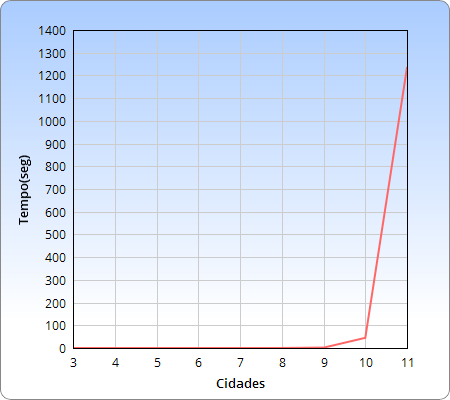
\includegraphics[width=6cm]{exato.png}
   \end{figure}
\begin{table}[ht]
\centering
\label{Exato}
\begin{tabular}{|ll|}
\hline
Exato                        &            \\ \hline
\multicolumn{1}{|l|}{Matriz} & Tempo      \\ \hline
\multicolumn{1}{|l|}{3}      & 0.003 s    \\ \hline
\multicolumn{1}{|l|}{4}      & 0.002 s    \\ \hline
\multicolumn{1}{|l|}{5}      & 0.003 s    \\ \hline
\multicolumn{1}{|l|}{6}      & 0.003 s    \\ \hline
\multicolumn{1}{|l|}{7}      & 0.017 s    \\ \hline
\multicolumn{1}{|l|}{8}      & 0.099 s    \\ \hline
\multicolumn{1}{|l|}{9}      & 1.876 s    \\ \hline
\multicolumn{1}{|l|}{10}     & 45.235 s   \\ \hline
\multicolumn{1}{|l|}{11}     & 1236.984 s \\ \hline
\end{tabular}
\end{table} 
   
%****************************************************************************************************************************************   
 \subsection{NN}
	O algoritimo tem como sua funcionalidade obter a cidade mais próxima da última visitada,assim "viajando" por todas as cidades com uma rota válida.É um algoritimo bem rápido mas que não traz um resultado excelente. 
 
 Foi um algoritimo bem simples de implementar com o seu codigo bem visual, como se o vetor trajeto estivesse se locomovendo na matriz pelas suas colunas somando os custos.   
\\\\\\\\\\\\gráfico de tempo por tamanho:
\begin{figure}[!htb]
  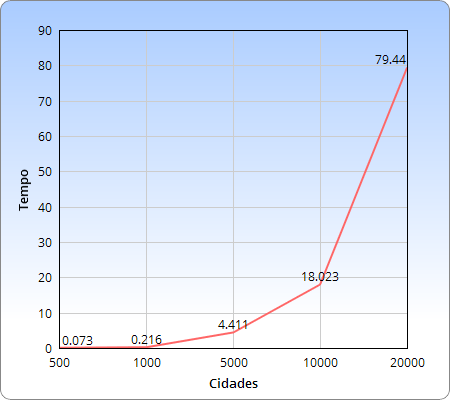
\includegraphics[width=6cm]{nn.png}
  \end{figure}
\begin{table}[ht]

\centering
\label{nn}
\begin{tabular}{|ll|}
\hline
nn	                         &          \\ \hline
\multicolumn{1}{|l|}{Matriz} & Tempo    \\ \hline
\multicolumn{1}{|l|}{500}    & 0.073 s  \\ \hline
\multicolumn{1}{|l|}{1000}   & 0.216 s  \\ \hline
\multicolumn{1}{|l|}{5000}   & 4.411 s  \\ \hline
\multicolumn{1}{|l|}{10000}  & 18.023 s \\ \hline
\multicolumn{1}{|l|}{20000}  & 79.44 s  \\ \hline
\end{tabular}
\end{table}
%****************************************************************************************************************************************
   \subsection{opt}
	Visto os possíveis resultados ruins providos do NN,o 2-opt,como algoritimo de melhoramento,tenta obter resultados mais pertos do caminho perfeito através de várias comparações que ele faz no decorrer do programa.
	Pudemos obter resultados melhores através dele,mas ele diminuiu o "range" de cidades capazes de calcular.
     \\\\gráfico de tempo por tamanho: 
   
   \begin{figure}[!htb]
   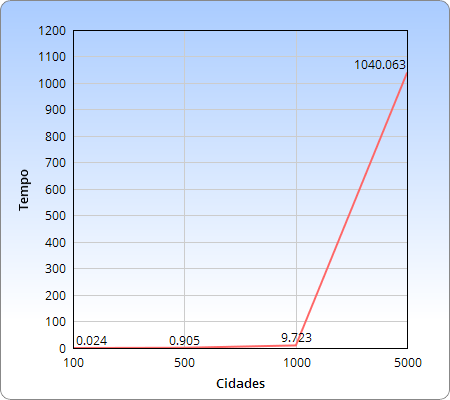
\includegraphics[width=6cm]{opt.png}
   \end{figure} 
\begin{table}[ht]
\centering
\label{opt}
\begin{tabular}{|ll|}
\hline
opt                        &          \\ \hline
\multicolumn{1}{|l|}{Matriz} & Tempo    \\ \hline
\multicolumn{1}{|l|}{100}    & 0.024 s  \\ \hline
\multicolumn{1}{|l|}{500}   & 0.905 s  \\ \hline
\multicolumn{1}{|l|}{1000}   & 9.723 s  \\ \hline
\multicolumn{1}{|l|}{5000}  & 1040.063 s \\ \hline
\end{tabular}
\end{table}
%****************************************************************************************************************************************  
   \subsection{Convex Hull}
   O algoritmo Envoltório Convexo (Convex Hull) tem como finalidade gerar um polígono convexo de forma que todos os pontos estejam dentro ou no perímetro do mesmo. Após isto, deve-se inserir todos os pontos interiores ao polígono, formando garantidamente uma aresta ao ponto mais próximo do envoltório.
 

\begin{table}[]
\centering
\label{Hull}
\begin{tabular}{|ll|}
\hline
Hull                         &       \\ \hline
\multicolumn{1}{|l|}{Matriz} & Tempo \\ \hline
\multicolumn{1}{|l|}{101}    & 0.003 \\ \hline
\multicolumn{1}{|l|}{1889}   & 0.193 \\ \hline
\multicolumn{1}{|l|}{11859}  & 1.355 \\ \hline
\end{tabular}
\end{table}
  
     grafico de tempo por tamanho: 
   
   \begin{figure}[!htb]
   \includegraphics[width=6cm]{genetico.png}
   \end{figure}
%****************************************************************************************************************************************  
 \subsection{Obsevação}
  Comparando os resultados das tres primeiros codigos observamos que exato se torna inviável muito rápido(matriz de 12 cidades), o NN 
  embora rapido não apresenta resultados bons em comparação ao melhor possivel, e o opt consegue resultados melhores embora reduza um pouco a quantidade de cidades máxima possíveis. \\
  Comparando os graficos temos:
  
     \begin{figure}[!htb]
   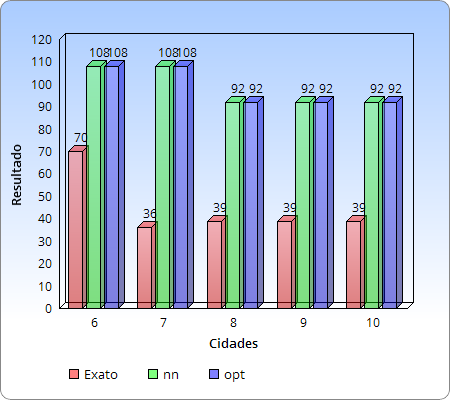
\includegraphics[width=6cm]{comparacao.png}
   \end{figure}

 \section{Conclusão}
 so observamos melhora do método opt em relacao a nn com uma quantidade de cidades relativamente grande,impossível de comparar com o método exato,o algorítimo Convex hull embora seja mais dificil de implementar em relação aos outros,traz resultados suficientemente bons támbem.
 
 \section{Bibliografia}
 
\begin{itemize}
  \item  http://latexbr.blogspot.com.br/2011/07/inserindo-figuras-no-latex.html
  
  \item http://www.tablesgenerator.com/
  
  \item http://www.chartgo.com/
  
  \item http://www.cplusplus.com/reference/cstdlib/srand/
  
  \item https://daemoniolabs.wordpress.com/2011/08/30/codigo-em-c-para-permutar-vetores/
\end{itemize}
 
\end{document}
